\chapter{LEVEL 2 @Problem 26 - 50}
\begin{chapquote}{Paul Dirac}
	``God used beautiful mathematics in creating the world.''
\end{chapquote}

\section{Problem 026 - Reciprocal cycles}
\begin{prob}
	\begin{figure}[htb!]
		\begin{center}
			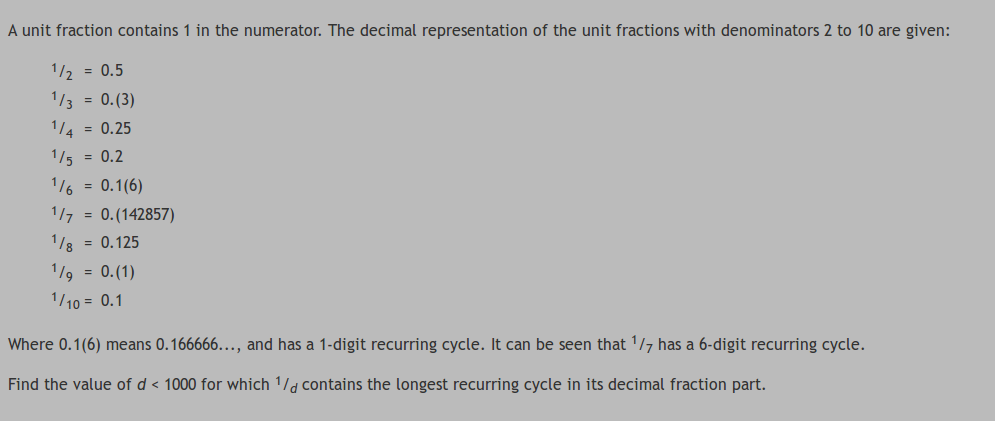
\includegraphics[scale = 0.4]{pic/026.png}
		\end{center}
	\end{figure}
\end{prob}
\begin{sol}
If $t$ is the period for number $p$, then
\begin{eqnarray}
10^{s + t} \equiv 10^s \mod p
\end{eqnarray}
If $p$ is relative prime with $2, 5$, then the above expression can be reduced to
\begin{eqnarray}
10^t \equiv 1 \mod p
\end{eqnarray}
Then brute force.
\code{code/026.py}
\end{sol}

\section{Problem 027 - Quadratic primes}
\begin{prob}
	\begin{figure}[htb!]
		\begin{center}
			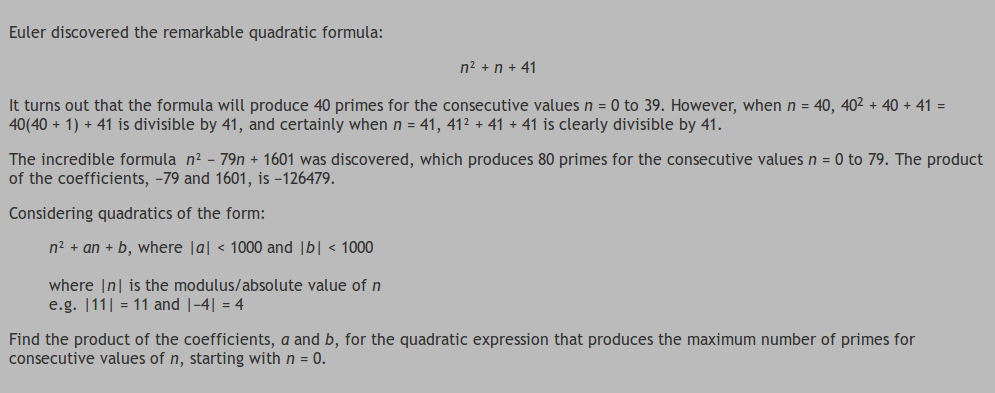
\includegraphics[scale = 0.4]{pic/027.png}
		\end{center}
	\end{figure}
\end{prob}
\begin{sol}
Brute force. But we know $b$ is a prime number between $0$ to $999$. Also we can see that when $n = b$, the result must be a compound, thus $n$ only goes from $0$ to at most $b - 1$.
\code{code/027.c}
\end{sol}

\section{Problem 028 - Number spiral diagonals}
\begin{prob}
	\begin{figure}[htb!]
		\begin{center}
			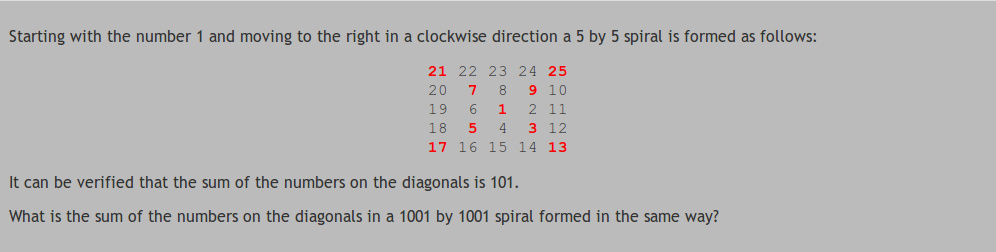
\includegraphics[scale = 0.4]{pic/028.png}
		\end{center}
	\end{figure}
\end{prob}

\begin{sol}

\end{sol}

\section{Problem 029}
\begin{prob}
	\begin{figure}[htb!]
		\begin{center}
			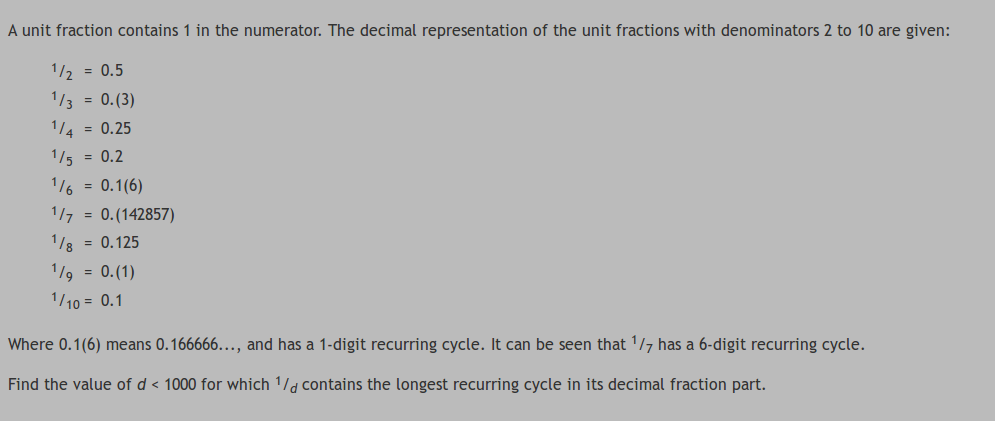
\includegraphics[scale = 0.4]{pic/026.png}
		\end{center}
	\end{figure}
\end{prob}

\section{Problem 030}
\begin{prob}
	\begin{figure}[htb!]
		\begin{center}
			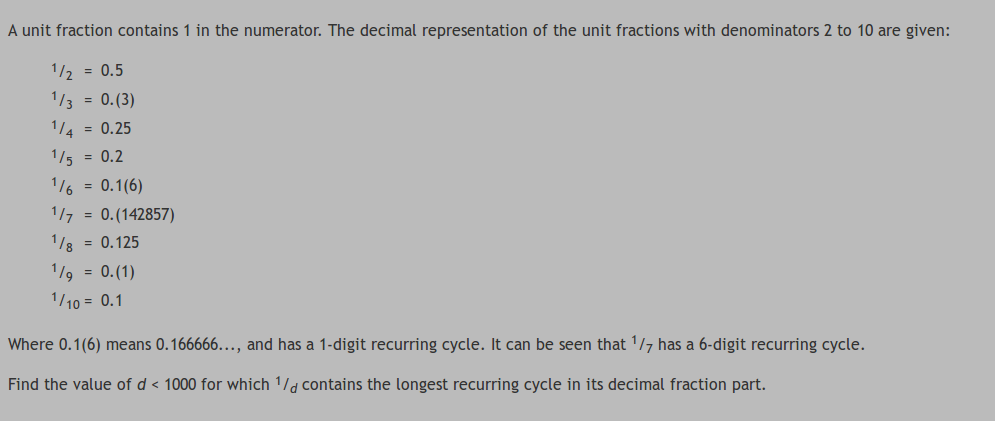
\includegraphics[scale = 0.4]{pic/026.png}
		\end{center}
	\end{figure}
\end{prob}

\section{Problem 031}
\begin{prob}
	\begin{figure}[htb!]
		\begin{center}
			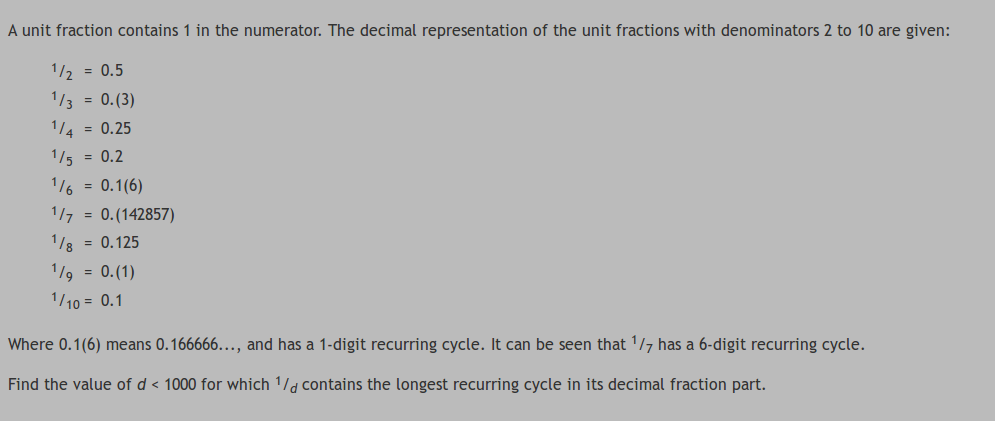
\includegraphics[scale = 0.4]{pic/026.png}
		\end{center}
	\end{figure}
\end{prob}

\section{Problem 032}
\begin{prob}
	\begin{figure}[htb!]
		\begin{center}
			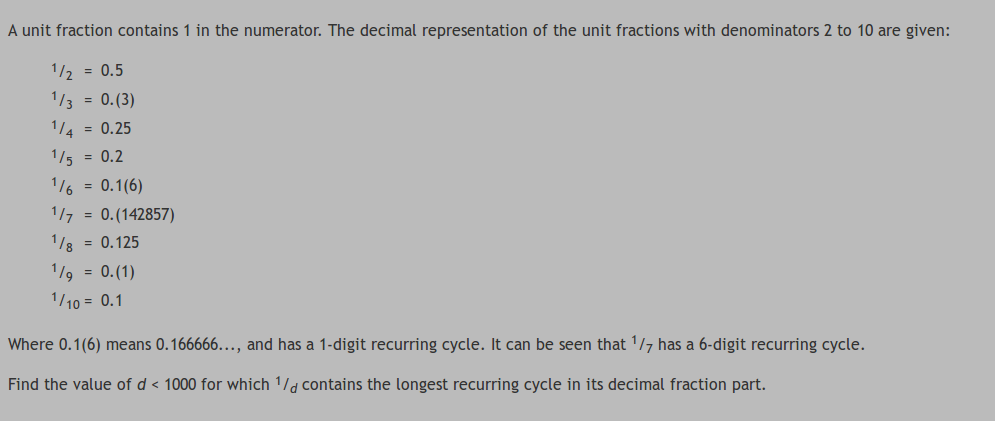
\includegraphics[scale = 0.4]{pic/026.png}
		\end{center}
	\end{figure}
\end{prob}

\section{Problem 033}
\begin{prob}
	\begin{figure}[htb!]
		\begin{center}
			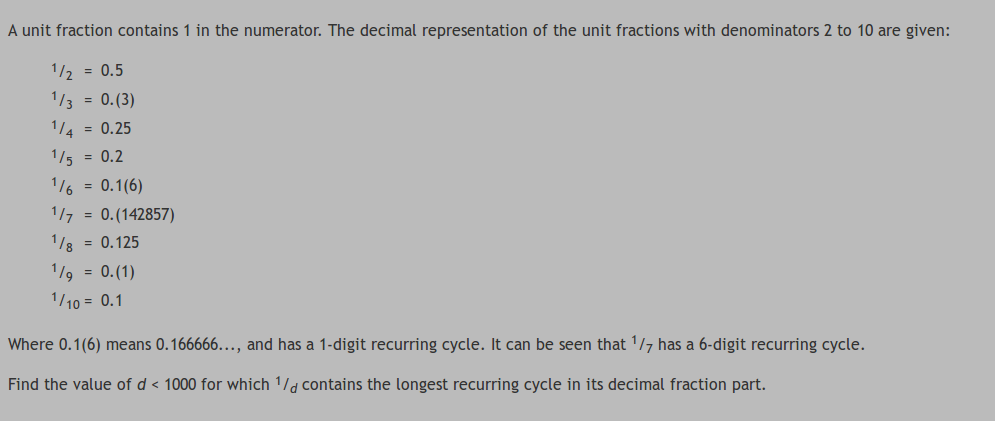
\includegraphics[scale = 0.4]{pic/026.png}
		\end{center}
	\end{figure}
\end{prob}
\section{Problem 034}
\begin{prob}
	\begin{figure}[htb!]
		\begin{center}
			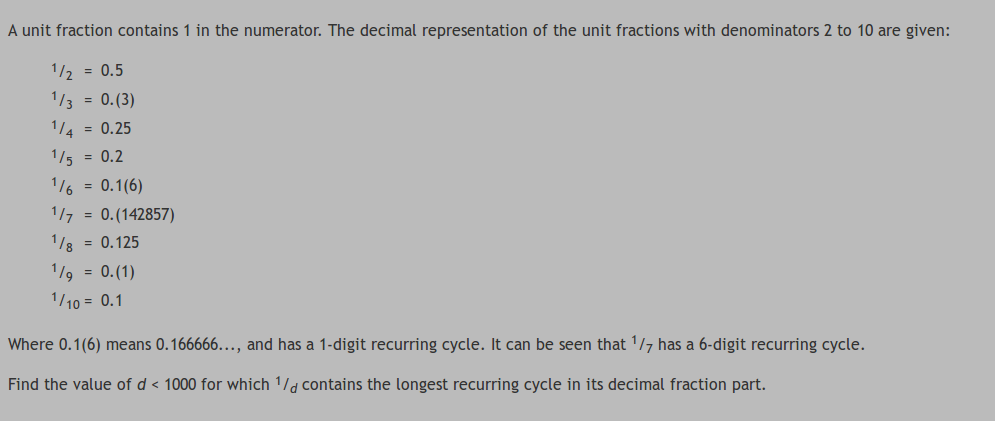
\includegraphics[scale = 0.4]{pic/026.png}
		\end{center}
	\end{figure}
\end{prob}
\section{Problem 035}
\begin{prob}
	\begin{figure}[htb!]
		\begin{center}
			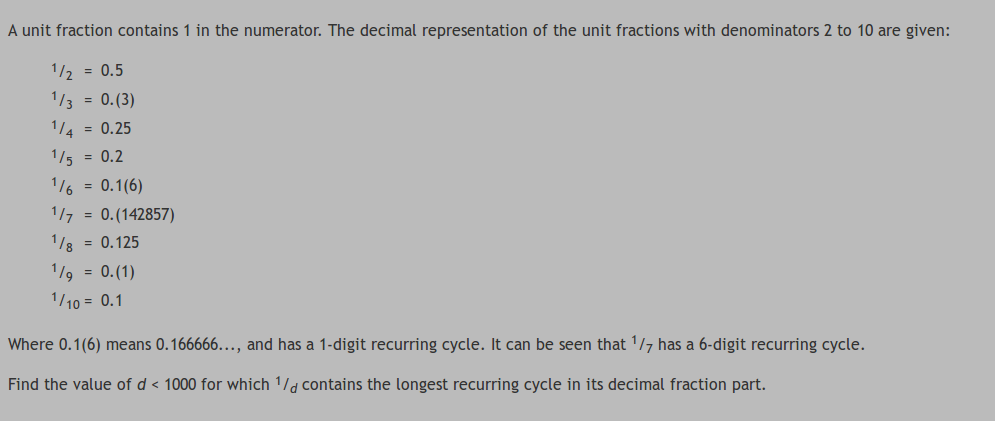
\includegraphics[scale = 0.4]{pic/026.png}
		\end{center}
	\end{figure}
\end{prob}
\section{Problem 036}
\begin{prob}
	\begin{figure}[htb!]
		\begin{center}
			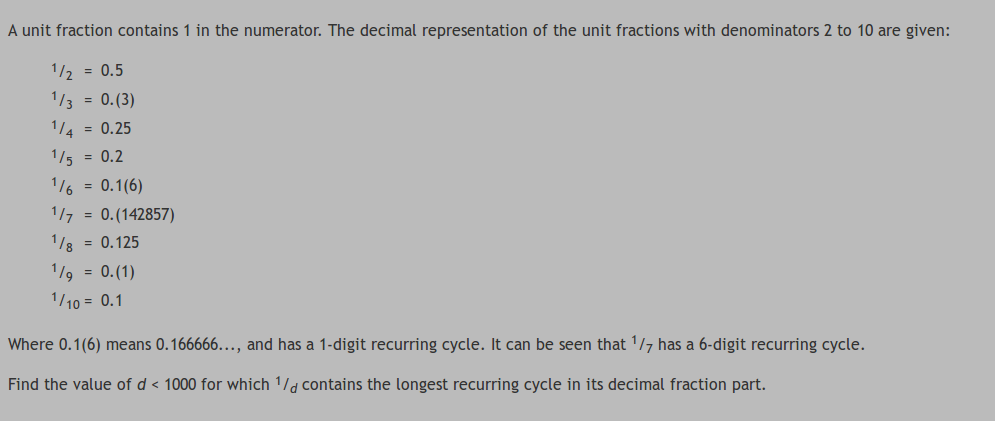
\includegraphics[scale = 0.4]{pic/026.png}
		\end{center}
	\end{figure}
\end{prob}
\section{Problem 037}
\begin{prob}
	\begin{figure}[htb!]
		\begin{center}
			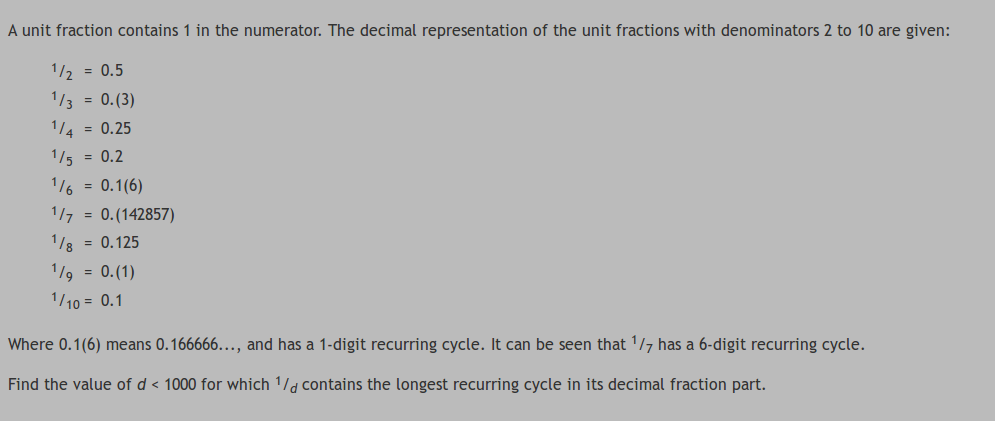
\includegraphics[scale = 0.4]{pic/026.png}
		\end{center}
	\end{figure}
\end{prob}
\section{Problem 038}
\begin{prob}
	\begin{figure}[htb!]
		\begin{center}
			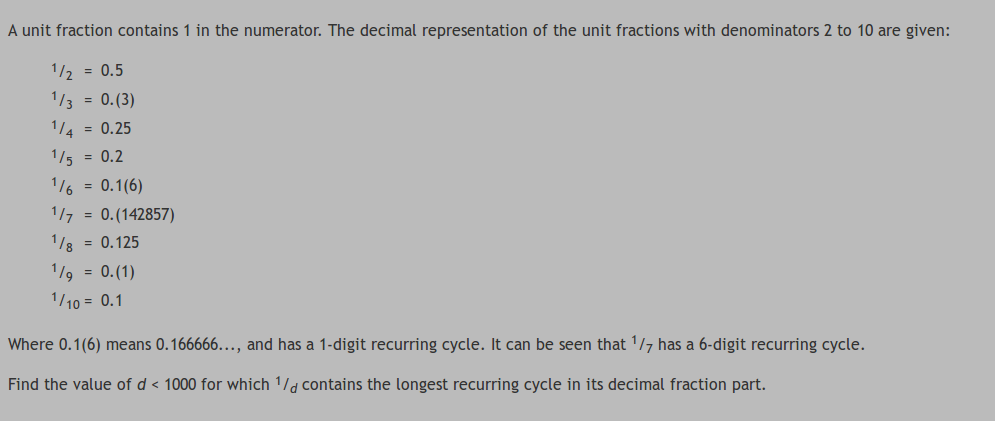
\includegraphics[scale = 0.4]{pic/026.png}
		\end{center}
	\end{figure}
\end{prob}
\section{Problem 039}
\begin{prob}
	\begin{figure}[htb!]
		\begin{center}
			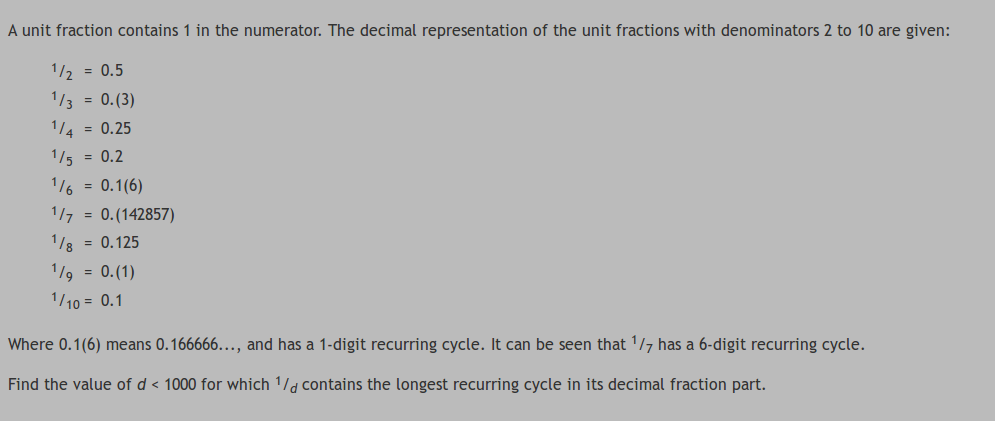
\includegraphics[scale = 0.4]{pic/026.png}
		\end{center}
	\end{figure}
\end{prob}
\section{Problem 040}
\begin{prob}
	\begin{figure}[htb!]
		\begin{center}
			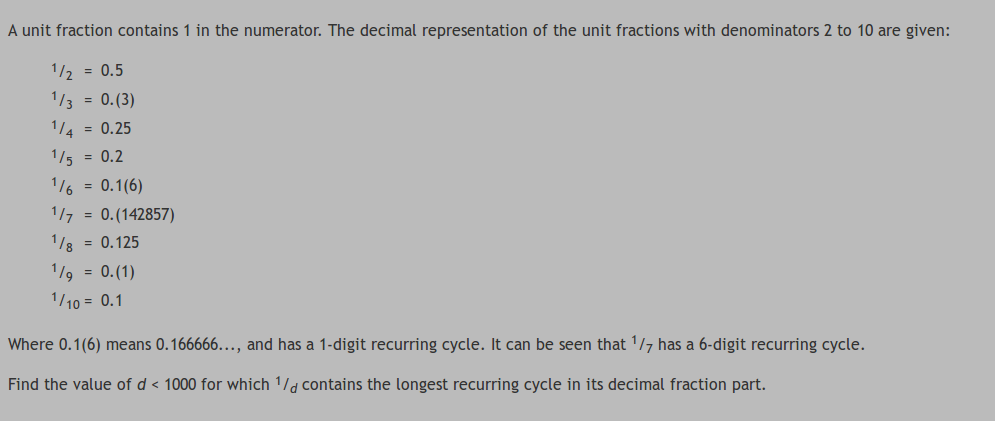
\includegraphics[scale = 0.4]{pic/026.png}
		\end{center}
	\end{figure}
\end{prob}